\documentclass[xcolor={usenames,dvipsnames,svgnames}]{beamer}
\usepackage[utf8]{inputenc}
\usepackage{graphicx}
\usepackage{subfigure}
\usepackage{hyperref}
\usepackage{mathtools}

%\AtBeginSection[] { \begin{frame} \frametitle{Table of Contents}
%\tableofcontents[currentsection] \end{frame} }
\usetheme{Berlin}
\usecolortheme{beaver}

% Custom math commands, other shortcuts
\newcommand{\tenexp}[1]{\times10^{#1}}
\newcommand{\dee}{\;\mathsf{d}}
\let\oldvec\vec
\renewcommand{\vec}[1]{\ensuremath{\mathbf{#1}}}
\newcommand{\evec}[1]{\ensuremath{\vec{e}_{#1}}} % standard basis vector
\newcommand{\norm}[2]{\ensuremath{\|#1\|_{#2}}}
\newcommand{\bignorm}[2]{\ensuremath{\left\|#1\right\|_{#2}}}
\newcommand{\infnorm}[1]{\ensuremath{\|#1\|_\infty}}
\newcommand{\reals}{\ensuremath{\mathbb{R}}}
\DeclareMathOperator{\Prob}{P}
% Physics Domain-Specific
\newcommand{\kB}{\ensuremath{k_\mathrm{B}}}
% General Shortcuts
\newcommand{\figref}[1]{Figure~\ref{#1}}
\newcommand{\secref}[1]{Section~\ref{#1}}

\newtheorem{assumption}{Assumption}

\begin{document}
\title[Genetic Networks]{Stochastic Simulation of Genetic Regulatory Networks}
\author[Max Veit]{Max Veit\\Advisor: Jorge Viñals}
\date[2014-03-12]{12 March 2014}
\institute[U of MN]{University of Minnesota}
\subject{Physics}

\frame{\titlepage}

\begin{frame} \frametitle{Outline}
%    \tableofcontents[part=1,pausesections]
	\tableofcontents
\end{frame}

\section{Introduction} % (fold)
\label{sec:introduction}
\begin{frame}
    \frametitle{Epigenetics}
    \begin{columns}[t]
        \begin{column}{0.5\textwidth}
            \begin{itemize}
                \item DNA is not the\\
                    whole story.
                \item Networks drive cell functions
                \item Special case:\\
                    biological clocks
                \item Synthetic versions\\
                    have been studied
                \begin{itemize}
                    \item Biological circuitry?
                \end{itemize}
            \end{itemize}
        \end{column}
        \begin{column}[T]{0.5\textwidth}
            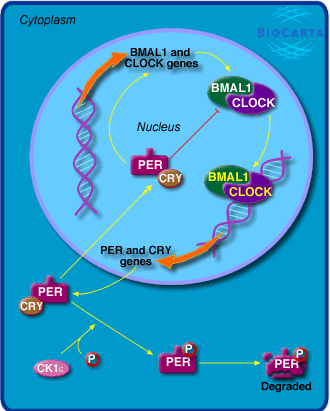
\includegraphics[width=0.85\textwidth]{h_circadianPathway.png}

            \small (Source: \cite{biocarta})
        \end{column}
    \end{columns}
\end{frame}

\begin{frame}
    \frametitle{Biochemical Networks}
    \begin{columns}[c]
        \begin{column}{0.5\textwidth}
            \begin{itemize}
                \item Systems of chemical reactions
                \item Reactions are interrelated
                \item Biological examples
            \end{itemize}
        \end{column}
        \begin{column}{0.5\textwidth}
            \begin{align*}
                \varnothing \xrightarrow{A} X \\
                X \xrightarrow {B} \varnothing
            \end{align*}
        \end{column}
    \end{columns}
\end{frame}

\begin{frame}
    \frametitle{Chemical Kinetics}
    What property of these reaction networks is most interesting for understanding genetic networks?
    \pause

    \emph{Time evolution.}
    \begin{itemize}
        \item How fast do the reactions run?
        \item Periodic, oscillatory behavior?
        \item Other behaviors (equilibrium, bistable, chaotic)?
        \item Bifurcations?
    \end{itemize}
\end{frame}

% section introduction (end)

\section{Modeling} % (fold)
\label{sec:modeling}

\begin{frame}
    \frametitle{Modeling}
    How do we model biochemical networks in order to study their behavior theoretically?
\end{frame}

\begin{frame}
    \frametitle{Reaction Rate Equations}
    \begin{itemize}
        \item Continuum limit
        \item Standard approach for large systems
        \item Turn chemical equations into differential equations
        \item Solve using standard techniques
    \end{itemize}
    \pause
    Example:
    \begin{columns}[c]
        \begin{column}{0.45\textwidth}
            \begin{align*}
                \varnothing \xrightarrow{A} X \\
                X \xrightarrow {B} \varnothing
            \end{align*}
        \end{column}
        \begin{column}{0.1\textwidth}
            \huge $\mapsto$
        \end{column}
        \begin{column}{0.45\textwidth}
            \begin{center}
                $\frac{\dee x(t)}{\dee t} = A - B x(t)$

                so

                $x(t) = \frac{A}{B} + x(0) e^{-B t}$
            \end{center}
        \end{column}
    \end{columns}
\end{frame}

\begin{frame}
    \frametitle{Why is a stochastic description necessary?}
    On a cellular scale, things look different:
    \hfill
    \begin{columns}[c]
        \begin{column}{0.5\textwidth}
            (Plot of concentration oscillating about a mean)
        \end{column}
        \begin{column}{0.5\textwidth}
            \begin{itemize}
                \item Concentrations oscillate about steady-state values
                \item Concentrations are discrete (``populations'')
                \item Noise is essential feature of some systems
            \end{itemize}
        \end{column}
    \end{columns}
\end{frame}

\begin{frame}
    \frametitle{Stochastic Chemical Kinetics}
    Different approach: Describe the evolution of a \emph{probability distribution}.
    
    Time evolution described by the chemical master equation (CME).
    \pause

    Derived from the premise:
    \begin{assumption}[\cite{gillespie-07}]
        The probability that a given reaction $R_j$ will occur somewhere in the system volume within the infinitesimal time interval $[t, t+\dee t]$ depends only on the current state $\vec{x}$:
        \[
            P_j(\vec{x}, [t, t+\dee t]) = a_j(\vec{x})\dee t
        \]
    \end{assumption}

    $a_j(\vec{x})$: ``Propensity''
\end{frame}

\begin{frame}
    \frametitle{Notes on Chemical Master Equation}
    \begin{itemize}
        \item Describes a \emph{Markovian} process\\
            (evolution depends only on current state)

        \item Assumptions about system:
        \begin{itemize}
            \item Reactions occur instantaneously
            \item Well-stirred system
            \item Ideal gas or dilute solution (!)
        \end{itemize}
    \end{itemize}
\end{frame}

\begin{frame}
    \frametitle{Abstraction: Delayed Reactions}
    \begin{itemize}
        \item Biological processes consist of many small reactions
        \item Often don't want to simulate every step
        \item Abstract sequence into one reaction with a delay
    \end{itemize}
    (Figure: Delayed reactions)
    \pause

    \emph{Note}: delay breaks Markovian property!
\end{frame}

% section modeling (end)

\section{Methodology} % (fold)
\label{sec:methodology}

\begin{frame}
    \frametitle{Methodology}
    How do we solve the chemical master equation to obtain the time evolution of a stochastic system?
\end{frame}

\begin{frame}
    \frametitle{Stochastic Simulation Algorithm (SSA)}
    Introduced by Daniel Gillespie, 1976.

    Features:
    \begin{itemize}
        \item Monte Carlo approach
        \item Generates trajectories that\\
            \emph{sample} the probability distribution
        \item Simulates a sequence of reactions
        \begin{itemize}
            \item Probability distributions\\
                for next reaction known (propensities).
            \item Reaction type and time\\
                randomly chosen.
        \end{itemize}
    \end{itemize}
    Typically treat trajectories statistically.
\end{frame}

\begin{frame}
    %TODO Call this the ``concentration space'' instead?
    \frametitle{Undersampling the Phase Space}
    Trajectories spend lots of time in certain regions of space.

    Other regions get ignored.

    (Figure: Sampling a bimodal distribution)
\end{frame}

\begin{frame}
    \frametitle{Resampling Using a Weighted Ensemble}
    Idea: Assign each trajectory in the ensembe a weight $w_j$.\\
    Divide the phase space into bins.
    \begin{columns}[c]
        \begin{column}{0.5\textwidth}
            \begin{enumerate}
                \item Run trajectories for time $t_s$.
                \item Pause trajectories.\\
                    In each bin:
                \pause
                \begin{itemize}
                    \item If not enough trajectories,\\
                        split some.
                    \pause
                    \item If too many,\\
                        combine some.
                    \pause
                    \item In any case,\\
                        \emph{conserve weight} in bin.
                \end{itemize}
                \pause
                \item Repeat.
            \end{enumerate}
            \pause
            Statistical \emph{resampling} procedure.
        \end{column}
        \begin{column}{0.5\textwidth}
            (Sequence of images to illustrate weighted ensemble)
        \end{column}
    \end{columns}
\end{frame}

\begin{frame}
    \frametitle{Conceptual Issues}
    SSA does not use \emph{uniform} timesteps. How to pause?

    (Figure illustrating non-uniform timesteps)

    Not a problem \emph{if} system is Markovian.
\end{frame}

\begin{frame}
    \frametitle{Delays Complicate Things Further}
    (Figure illustrating delayed reactions)

    From where is delay measured?
\end{frame}

\begin{frame}
    \frametitle{(Partial) Resolution}
    \begin{itemize}
        \item Physical standpoint: trajectory vs. system
        \item Trajectory remains in given state until next reaction
        \item Not \emph{inaccurate} resampling, just suboptimal\ldots
    \end{itemize}
\end{frame}

% section methodology (end)

\section{Preliminary Results}

\begin{frame}
    \frametitle{Delayed-Degradation System}
    \begin{columns}[c]
        \begin{column}{0.5\textwidth}
            \begin{align*}
                \varnothing \xrightarrow{A} X \\
                X \xrightarrow{B} \varnothing \\
                X \xRightarrow[(\tau)]{C} \varnothing
            \end{align*}

            Common model system
        \end{column}
        \begin{column}{0.5\textwidth}
            (Plot of DPD time evln)
        \end{column}
    \end{columns}
\end{frame}

\begin{frame}
    \frametitle{Numerical Evidence on Resampling}
    (Plot of Gaussian or delayed production-degradation system)
\end{frame}

%TODO More complex biological clocks: If plot available, show it.

\begin{frame}
    \frametitle{Upcoming Goals: Modeling Cells}
    Cells don't meet assumptions used by the SSA.

    Relax some assumptions:
    \begin{itemize}
        \item Crowded environment: modify reaction rates
        \item Inhomogeneity: introduce diffusion
    \end{itemize}
\end{frame}

\begin{frame}
    \frametitle{Summary and Project Goals}
    \begin{itemize}
        \item Adapt weighted-ensemble SSA for delays
        \item Apply simulation to common model systems
        \begin{itemize}
            \item Study system properties
            \item Validate/challenge common assumptions
        \end{itemize}
        \item Use simulation on more complex systems
        \item More realistically model cells
    \end{itemize}
\end{frame}

\begin{frame}[plain]

\hfill
    \begin{beamercolorbox}[rounded=true, center, shadow=true,wd=6cm]{title}
        \huge Questions?
    \end{beamercolorbox}
\hfill\hfill

\end{frame}

\appendix

\begin{frame}
    \frametitle{References}
    \begin{thebibliography}{9}
        \bibitem{biocarta} ``Biocarta - Charting Pathways of Life.'' \url{http://www.biocarta.com/genes/index.asp}.
        \bibitem{gillespie-07} D. Gillespie, Annu. Rev. Phys. Chem. \textbf{58}, 35-55 (2007).
        
    \end{thebibliography}
\end{frame}

\end{document}
